\section{Proposed Method}
In this section, we first describe how we represent text as a graph using the dependency parse tree. We then convolve over this dependency graph using a graph convolutional framework (DepGCN) to compute a text embedding used for offensive language detection task. Further, we describe our novel GCN based architecture that exploits the user social graph to augment the text embeddings.

\subsection{Graph representation of Text}
We use the dependency parse tree to induce a graph on a sentence. Specifically, a graph $G = < V, E > $ is represented as a collection of vertices $V$ and as a set of edges $E$ between these vertices. Thus, to compute the graphical representation of the sentence, we treat each word as a vertex, with syntactic dependencies between words corresponding to an edge. Now, for this graph $G$, $\textbf{A}$ represents the Adjacency matrix where $A_{ij} = 1$ if there is a dependency relation between word $i$ and $j$ and $0$ otherwise. We also connect each word to itself such that $A_{i,i}$ = 1; $\forall i \in V$. Although syntactic dependencies are directed, we treat these dependency edges as undirected, resulting in a symmetric matrix\footnote{Similar to \cite{zhang-graph}, we observed a performance dip when using each edge direction as a separate graph.}.

Graph Convolution Networks (GCN) are recently proposed to compute vertex embeddings in a graph by convolving over each vertex's local neighborhood \cite{kipf2016semi}.

The convolution operation for vertex $i$ in layer $k$ in GCN is defined as follows,

\begin{align}
    h_i^{k+1} &= \sigma \left ( \sum_{j = 1}^{|V|}  \tilde{A}_{ij} W^k h_j^k + b^k  \right ) \\
    &= \sigma \left ( \frac{ \sum\limits_{j \in \mathcal{N}(i) \cup i} W^k h_j^k} {d_i} + b^k  \right )
\end{align}
where $\mathbf{\tilde{A}} = D^{-1/2}\mathbf{A}D^{1/2}$ is the normalized Adjacency matrix with $D$ being the degree matrix. $h_i^{k+1}$ represents the vertex embeddings at layer $k+1$, with $h_i^0$ being initialized with the vertex features. In our case, we use pretrained word embeddings as the initial features.
$W^k, b^k$ are learnable weight and bias parameters of layer $k$ and $\sigma$ represents the ReLU function. $\mathcal{N}(i)$ represents the vertex \emph{i}'s neighborhood while $d_i = \sum {D}_i$ represents the vertex degree.

Now, assume that $W^k = \mathbf{{I}}$ with $b^k = 0$ and $\sigma(.)$ as an identity function. The updated vertex embedding at layer $k+1$ will be,
\begin{align}
    h_i^{k+1} &= \frac{ \sum\limits_{j \in \mathcal{N}(i) \cup i} h_j^k} {d_i}
\end{align}
It is thus easy to verify that the convolution operation updates the vertex embeddings at layer $k+1$ to be the average embeddings of the vertex's neighborhood and the vertex itself from the previous layer, $k$. In our dependency graph, applying graph convolution operation will augment each word's embedding with its syntactic neighbors.
Thus, convolution helps to contextualize the word embeddings, where the word's syntactic relationships define the context. Notice that it is different from the sequential models (like LSTM or CNN), where the adjacent words in the sentence define the context.

Consider the sample tweet in Figure \ref{fig:parser}, first, \textit{ill} will be augmented with its surrounding adverbs \textit{mentally} and \textit{just} (\cref{eq:sample}). In turn, these updated embeddings of \textit{ill} will be propagated when computing embeddings of the noun \textit{people} in addition to the subject \textit{Transgenders}.
\begin{align}
      \label{eq:sample}
      h_{ill} &= f_{gcn}(h_{mentally}, h_{just}, h_{ill}) \\
      h_{people} &= f_{gcn}(h_{ill}, h_{transgenders}, h_{people})
\end{align}
However, in sequential models with a fixed window, the attack \textit{ill} will be too far from the subject \textit{Transgenders}.

Further, by stacking such $k$ convolution layers, we can propagate the vertex embeddings to its k-hop neighborhood \cite{kipf2016semi}. For our experiments, we did not see any further improvements after two layers. This could be because, as we are dealing with a short text, the resulting parse tree is shallow.

\subsection{Sentence representation}
In the previous section, we computed contextualized word embeddings using syntactic relationships. However, we still need to aggregate these node embeddings to compute a graph-level embedding (sentence in our case). In particular, we perform masked pooling over the learned word embeddings from the last layer ($K$) to compute a sentence embedding. We only pooled over non-terminal words or intermediary nodes in the dependency parse tree (i.e. $\vert A_{i} \vert > 2$). We ignored the leaf words or words linked to only one other word as their word embeddings are relatively unchanged (because of less number of neighbors) after the convolution as compared to other intermediary nodes with more neighbors. Thus, when we perform pooling over all the words, leaf words will skew the final result even though they are not always important. We tried different variants of pooling (average and min), but max-pooling performed the best (\cref{eq:max}) for our case.
\begin{align}
  \label{eq:max}
    h_G &= \max_{i \in V'} (h_i^K) \; s.t. \vert A_{i} \vert = 2
\end{align}
Further, these sentence embeddings are fed through fully connected layers followed by a sigmoid ($\sigma$) to compute final class score (\cref{eq:class}) for the sentence.
\begin{equation}
    c_G =   \sigma (f_{MLP}(h_G)); c_G \in \mathbf{R}^C
    \label{eq:class}
\end{equation}
Here, $C$ represents the total number of classes.

\subsection{Embedding variants}
As we deal with noisy text, there can be ill-formed words and grammatically incorrect sentences that can lead to incorrect parse trees. Thus, to overcome these potential errors, we feed the initial word embeddings ($h_i^0$) to a BiLSTM module. The BiLSTM module helps to aid in word disambiguation by encoding adjacent words in the sentence.

\begin{figure}
    \centering
    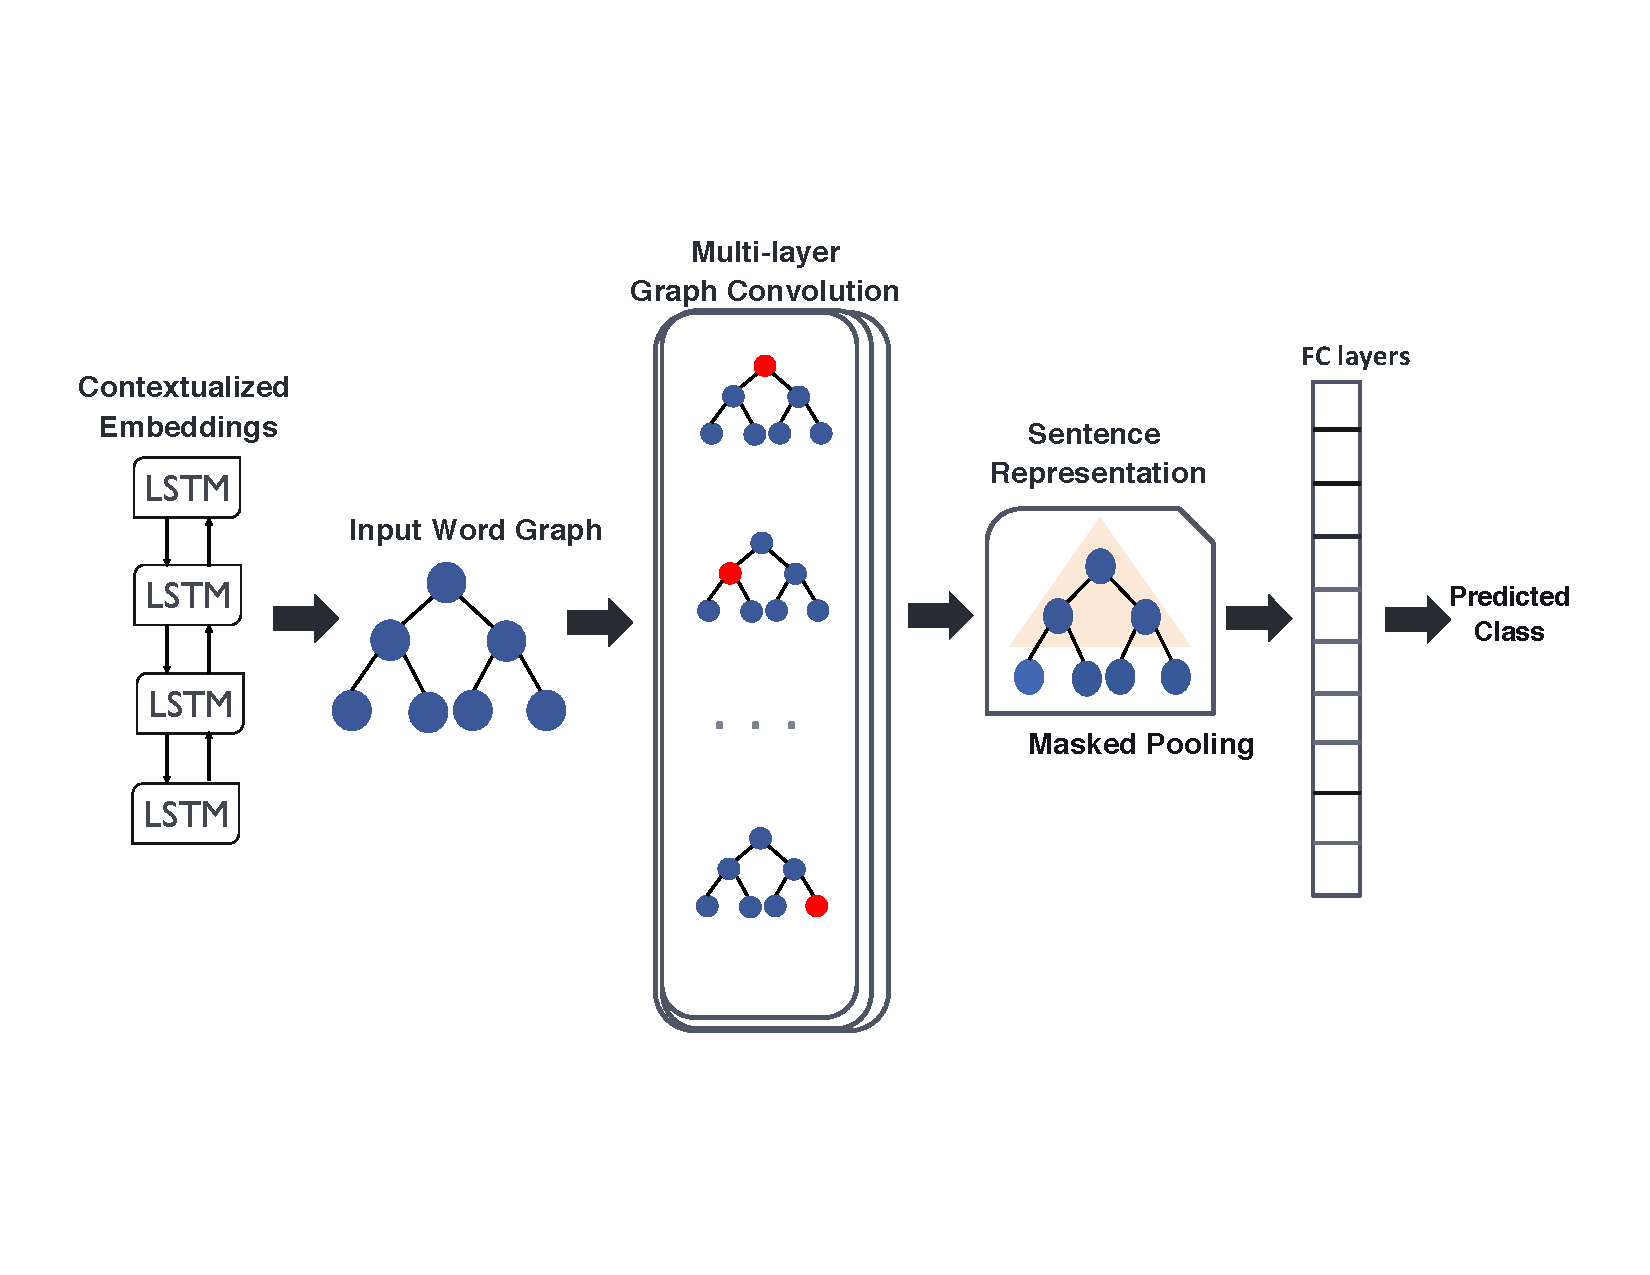
\includegraphics[scale=0.6]{figures/architecture_key.pdf}
    \caption{Overview of our proposed model}
    \label{fig:arch}
\end{figure}
The final architecture of our dependency graph convolution network (DepGCN) is depicted in \Cref{fig:arch}.
\subsection{User Features}
\citet{mishra2019abusive} observed that only a small set of users were responsible for most of the offensive tweets in the \citet{waseem-hovy-2016} dataset. In a similar analysis on tweets posted in response to President Obama's re-election, \citet{racist_article} found that most of the racist tweets came from only a group of states. Thus, it shows that determining the author of the tweet will be beneficial for automated offensive language detection.

Further, prior studies have shown that user behavior is influenced by their friends in online social networks leading to similar behavior(user homophily) of connected users \cite{homophily, social_influence}.
To empirically verify this in \citet{waseem-hovy-2016} dataset, we computed the average cosine similarity between the class distribution of a user's tweets and their friends' tweets. We observed a high similarity value of \emph{0.80}, indicating similar tweeting behavior between connected users. In other words, this high value shows that users connected to offensive users tend to follow suit. Thus, modeling the influence of user's social connections can potentially improve our understanding of user behavior.
We thus extend our proposed model to augment the sentence embeddings obtained from DepGCN with the social embeddings capturing user and her friends' tweeting behavior.

To this end, we use the follower followee relationship of each user in our dataset from Twitter\footnote{Thanks to authors of \cite{mishra2019abusive} for providing the user social relationship data.}. Similar to the dependency graph, we create a social graph and represent each user as a vertex, and the edges represent the follower relationship. For our experiments, we treat the follower-followee relationship as equivalent. We believe that it is a reasonable assumption, as in general, follower-followee relationships are often reciprocal, and our dataset does not contain any celebrities (skewed ratio of followers vs. followee).

To capture the user's tweeting behavior, we first compute user embeddings ($e_u$) as the average of the sentence embeddings obtained from DepGCN, for all the tweets authored by the user (\cref{eq:user}).
\begin{align}
\label{eq:user}
    e_u &= \frac {\sum_T h_T} {\vert \mathcal{A}(u) \vert}; \forall T \in \mathcal{A}(u)
\end{align}
$\mathcal{A}(u)$ represents all the tweets authored by the user $u$.

To capture the effect of homophily, we perform graph convolution operation on the user's social graph with these user embeddings being used as initial vertex features ($h_u^0$).

In the first layer of the graph convolution, we project these user embeddings to a $C$ dimensional vector to learn the user's prior distribution per class. It is not correct to classify each user or all her tweets to be abusive or not. Therefore, we learn a class probability for each user, which indicates her likelihood of posting an offensive tweet.

In the subsequent layers, we propagate these class priors through the user's social network.
\begin{equation}
    h_u^k = \sigma \left ( \frac{ \sum_{v \in \mathcal{N}(u) \cup u} W^k h_v^k} {d_u} + b^k  \right )
\end{equation}
where $\mathcal{N}(u)$ denotes the friends of user $u$.

\begin{align}
    h_S &= \sigma (h_u^K) \\
    c_F &= f_{MLP}( [h_G, h_S] )
\end{align}
where $h_S \in R^C$ are social embeddings for user who tweeted the tweet.
Finally, we concatenate the text and social embeddings for each tweet and compute the final class probability.
The final architecture of UserGCN with our DepGCN is depicted in \Cref{fig:userarch}.

\begin{figure}
    \centering
    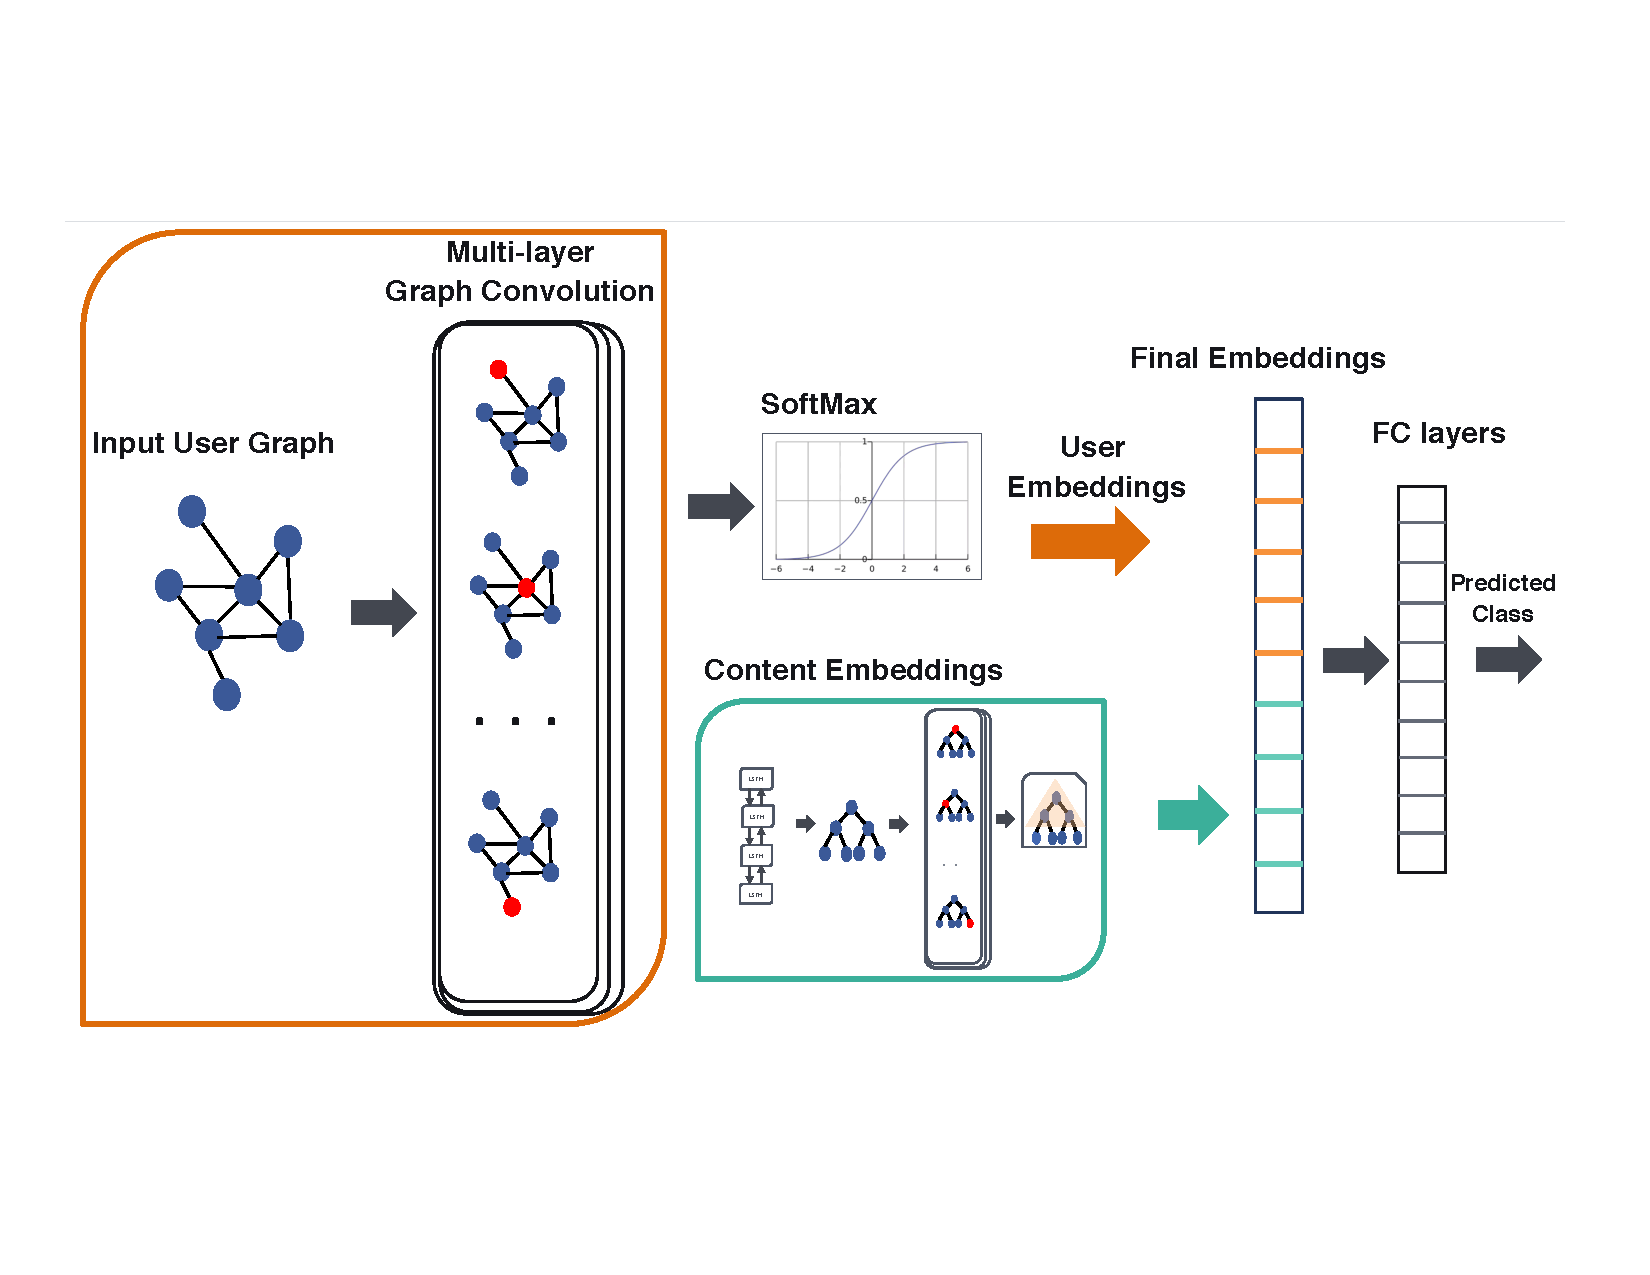
\includegraphics[scale=0.6]{figures/Userarchitecture_key}
    \caption{Overview of our proposed model with user social graph}
    \label{fig:userarch}
\end{figure}
